\documentclass{article}
\usepackage{graphicx}
\usepackage[utf8]{inputenc}
\usepackage[T1]{fontenc}
\usepackage[francais]{babel}
\usepackage{layout}
\usepackage{caption}
\usepackage{subcaption}

\begin{document}
\begin{titlepage}
\begin{center}
\Huge Rapport TPA phase 2

\normalsize
\vspace{0.5cm}
\Large {\underline{ Groupe 3 Bleu : Sokoban} }

\vspace{1cm}

\normalsize
Basset Emilien , Goron Nathan, De La Rosa Louis-David, Demé Quentin

\vspace{1cm}
\begin{center}
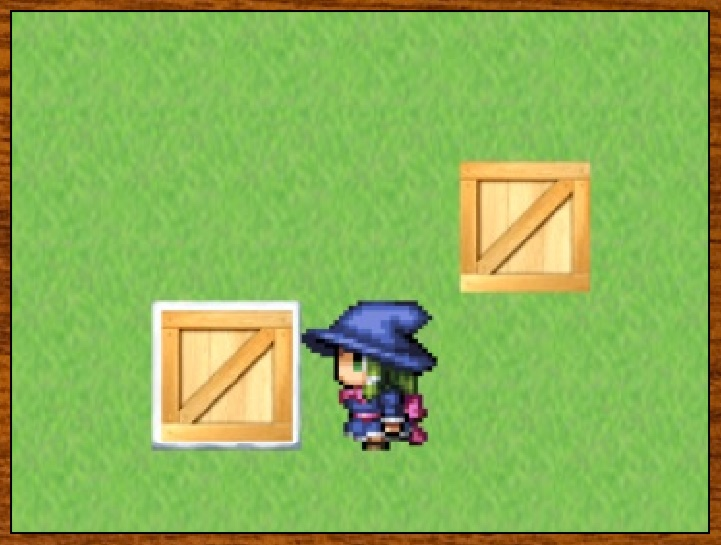
\includegraphics[scale=0.7]{img/main.jpg}
\end{center}
\vspace{3.5cm}
L2 informatique 2016-2017 Université de Caen Basse-Normandie
\end{center}
\end{titlepage}

\newpage
\tableofcontents

\newpage
\begin{center}
	\section{\underline{Introduction}}
	\vspace{2 cm}
	Parmi les projets proposés, nous avons fait le choix d’éviter les projets n’étant
pas des jeux de peur qu’ils limitent notre créativité et notre motivation quant a
son développement. Le jeu de Sokoban nous paraissait être un projet ambitieux
et intéressant de par la difficulté de l’implémentation de son IA de résolution automatique.
Il s'agissait donc de développer un Jeu de Sokoban : Un jeu de puzzle dans
lequel un personnage déplace un certains nombres de caisses sur des emplacements
dans un niveau fermé, le joueur gagne la partie si il parvient à boucher
tous les emplacements avec les caisses.

Après avoir songé à l’utilisation du moteur de jeu Unreal Engine, nous avons
décidé de développer ce projet en Python avec l’aide de la librairie PyGame
qui offre une grande liberté dans le développement de l'interface graphique ainsi que de nombreuses
méthodes facilitant les mécaniques de fonctionnement de base d’un jeu.

\end{center}

\newpage
\begin{center}
	\section{\underline{Cahier des Charges}}
	\vspace{2 cm}
	\end{center}
		\subsection{Résumé des objectifs , principe du jeu:}
		\vspace{1cm}
		Dans le cadre de L'UE "Travaux personnels encadrés" , il s'agira de développer un jeu de sokoban : Un joueur est introduit dans un niveau constitué de caisses et d'obstacles , il doit pousser toutes les caisses sans bloquer ces dernières afin de compléter le niveau.
		L'application sera agrémenté d'une fonctionnalité de résolution automatique dites anytime via un algorithme Astar ainsi que d'autres fonctionnalités additionnelles facultatives.
		
		
		\subsection{Pré-requis d'utilisation}
		\vspace{1cm}
		Le jeu fonctionnera sous n'importe quelle machine sous linux/windows munie de Python(2.7 a 3.5) ainsi que des modules Pygame et PIL .Le jeu sera intuitif d’utilisation , ne nécessitera aucune connaissance informatique particulière et sera donc accessible a tout type de public .

		\subsection{Recensement des fonctionnalités}
		\vspace{1cm}
			\subsubsection{Fonctionnalités obligatoires}
			Le jeu devra obligatoirement présenter un moteur de jeu permettant au joueur de se déplacer dans le niveau en respectant les règles(pousser les caisses , collisions avec les blocs non traversables ...).Le jeu sera également muni d'une fonctionnalité de résolution automatique anytime.
			\subsubsection{Fonctionnalités additionnelles}
			L'application se verra ajouter les fonctionnalités suivantes :
			\begin{itemize}
			\item Une interface graphique intuitive et simple d'utilisation , dotée d'un menu principal pour guider le joueur dans le choix du niveau et les autres options disponibles .
			\item Un set de plusieurs styles pour le personnage et le niveau 
			\item Une option de sauvegarde / chargement de partie
			\item Une fonctionnalité de retour arrière suite a un mouvement involontaire ou a une erreur dans un niveau 
			\end{itemize}
		\subsection{Découpage de l'application}
		\vspace{1cm}
	Le programme sera composé des modules suivants :
		\begin{itemize}
\item Le module sokoban qui servira de module "Init" au programme.
\item Le module classes qui comprendra toutes les classes et méthodes nécessaire
au fonctionnement du jeu.
\item Le module constantes stockant les instanciations d'objets ,les importations d’images pour les personnages
et les cases ainsi que les variables nécessaire pour les variations
de tailles de niveaux a l’écran.
\item Le module IA qui gérera l'exécution de l'algorithme Astar et de l'heuristique.
Ce découpage pourra être modifié en fonction des choix de fonctionnalités additionnelles.
\item Le module GUI qui assurera la communication entre le joueur et l'interface.
\item Le module sauvegarde qui permettra la sauvegarde et chargement d'une partie dans le dossier "/sauvegardes
\item Le module imagery qui permettra le redimensionnement des niveau dans la fenêtre en fonction de la taille de ceux-ci via la librairie PIL
		\end{itemize}

\newpage

\section{\underline{Explication du programme ; interface et  moteur de jeu}}


\vspace{1.5 cm}
\subsection{Moteur de jeu}

			\subsubsection{Le menu}
	L'une des principales modifications de l'interface lors de cette seconde phase n'est autre que l'ajout d'un menu interactif regroupant plusieurs options pour le joueur. Parmi ses options, on peut citer:
\begin{itemize}
\item Le bouton \textbf{Nouvelle Partie}, pour démarrer une partie.
\item Le bouton \textbf{Charger Partie}, pour reprendre une partie sauvegardée.
\item Le bouton \textbf{Option}, pour configurer certaines propriétés du jeu.
\item Un bouton \textbf{Quitter}, pour quitter le jeu.
\end{itemize}
De plus, le menu se charge de jouer une musique d'introduction pour le joueur. Tout cela est commandé par la fonction \textbf{collectionMenu()}, elle est sans arguments et se présente comme un hub, au sens ou elle fait communiquer les autre fonctions entre elles, tout en gérant elle-même certains points. \newline
Dans un premier temps la fonction se charge de placer les boutons et l'interface globale. Les boutons sont simplement des images que l'on vient coller sur l'interface. Pour finir, la fonction s'engage dans une boucle infinie en attendant un événement de la part de l'utilisateur. On obtient ainsi la fenêtre suivante: 
\begin{figure}[!h]
\centering
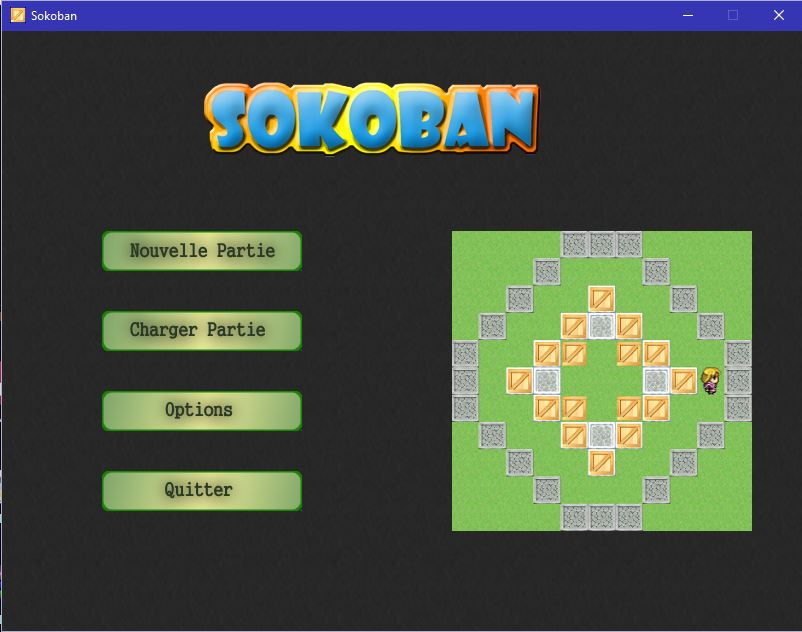
\includegraphics[scale=0.5]{img/menu-interface.jpg}
\caption{Menu du jeu Sokoban}
\end{figure}
\newline
		\subsubsection{Découpage et fonctionnement du moteur de jeu}
Notre moteur de jeu repose sur 5 classes:
\begin{itemize}
\item \textbf{Sprite} 
\item \textbf{Personnage }
\item \textbf{Caisse}
\item \textbf{Niveau}
\item \textbf{LevelCollection}
\end{itemize}
Les classes \textbf{Sprite}, \textbf{Personnage} et \textbf{Caisse} servent à représenter visuellement les objets suivants:
\begin{itemize}
\item \textbf{Personnage}: Classe représentant le personnage contrôlé par le joueur.
\item \textbf{Caisses}: Classe représentant les entités manipulable par le personnage.
\item \textit{Les murs}: Moteur de difficulté du jeu; Ils bloquent le déplacement des caisses et du personnage.
\item \textit{Les stèles}: représentent les emplacements sur lesquels le joueur doit placer les caisses.
\item \textit{Les cases vides}: Cases sur lesquelles le personnage et les caisses peuvent être déplacées.
\end{itemize}
La continuité du jeu est contrôlée par la variable \textit{continuer}. Celle-ci est établie à \textbf{1} au lancement du jeu et à \textbf{0} lorsque le joueur complète le niveau. Une fois la valeur nulle le jeu se bloque et il faut revenir au menu pour changer de niveau. \newline
			
Pour construire notre plan de jeu, nous avons choisi de décomposer notre niveau en 2 grilles nommées \textit{GameP} et \textit{GameO} contenant à elles deux les objets cités plus haut. La grille \textit{gameP}(game Plan)contient les cibles et les espaces vides tandis que la grille \textit{gameO}(game Obstacle) contient les murs, les caisses et le personnage. L'affichage du niveau consiste donc en la superposition des deux plans et permet ainsi une vérification de victoire plus facile à la fin du jeu : 
\begin{figure}[!h]
\centering
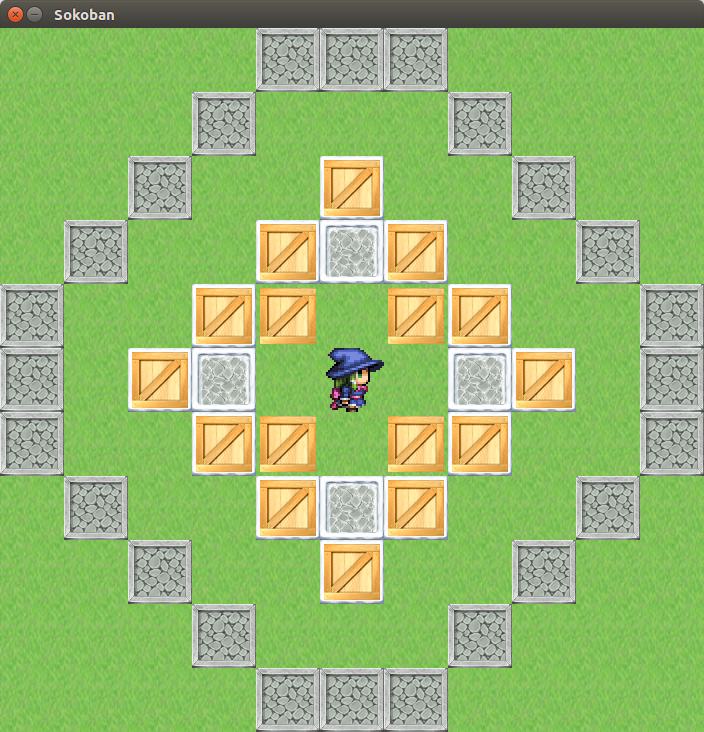
\includegraphics[scale=0.25]{img/05.png}
\caption{Apercu des deux grille superposées}
\end{figure}

\begin{figure}[!h]
\centering
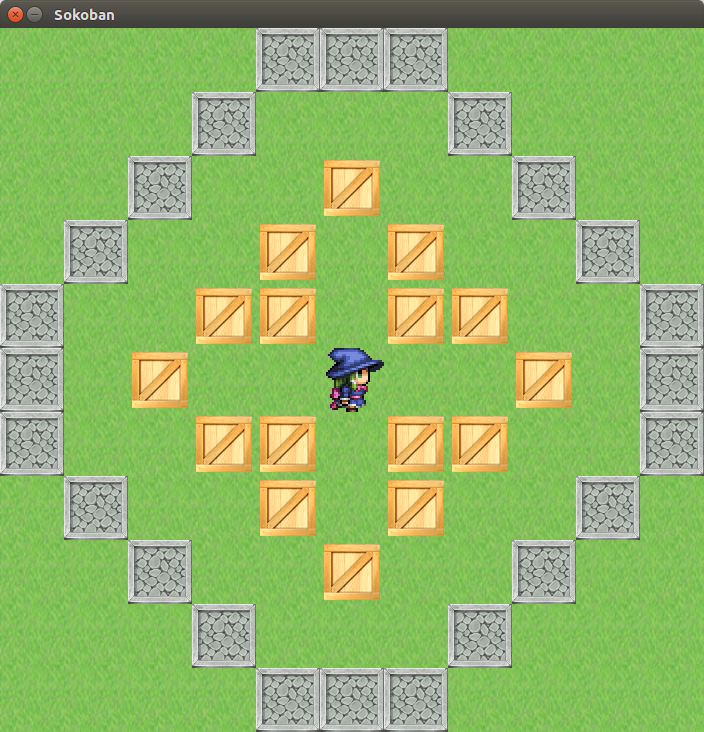
\includegraphics[scale=0.25]{img/06.png}
\caption{Apercu de la grille GameO}
\end{figure}

\begin{figure}[!h]
\centering
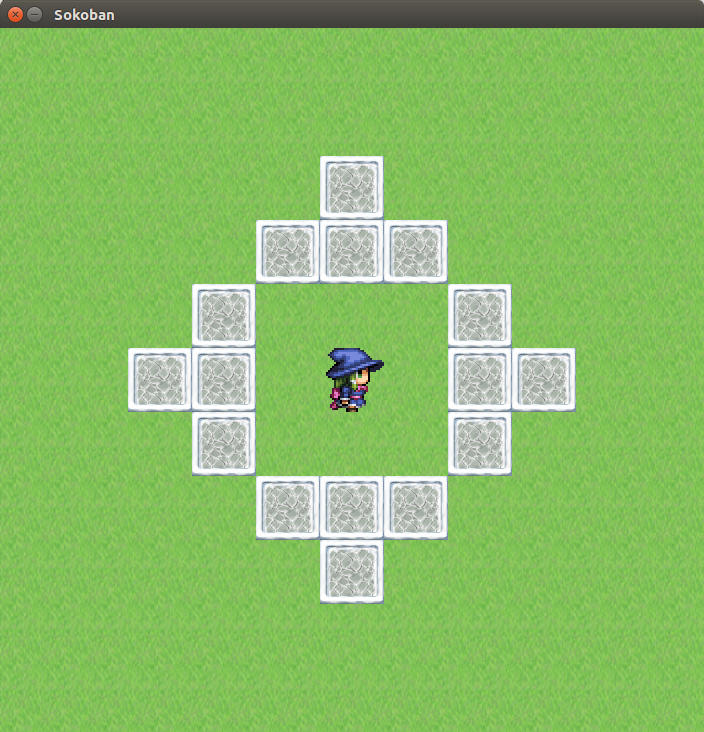
\includegraphics[scale=0.25]{img/07.png}
\caption{Apercu de la grille GameP}
\end{figure}
		\subsubsection{Communication jeu/utilisateur et utilisation du programme}
		
			Pour les déplacements du personnage nous utilisons la méthode event.key de PyGame qui permet de gérer des événements liées a l'utilisation du touches du clavier , 6 touches événement sont actuellement gérés : touche directionnelle droite(K-RIGHT : déplacement du personnage vers la droite) ,touche directionnelle gauche(K-LEFT : déplacement du personnage vers la gauche) ,touche directionnelle haut(K-UP : déplacement du personnage vers le haut) ,touche directionnelle bas(K-DOWN: déplacement du personnage vers le bas) ,   pavé numérique(KP-MULTIPLY: lance la résolution automatique du niveau avec Astar) et la touche échap(KP-ESCAPE : fermeture du jeu)
		\subsubsection{Restriction de déplacement du personnage}		
		Lorsque le joueur presse une des touche événement de déplacement citées plus ci-dessus , la méthode spéciale déplace() de la classe Personnage retournant un booléen est appelée pour vérifier si le déplacement est autorisé de la manière suivante:
\begin{figure}[!h]
\centering
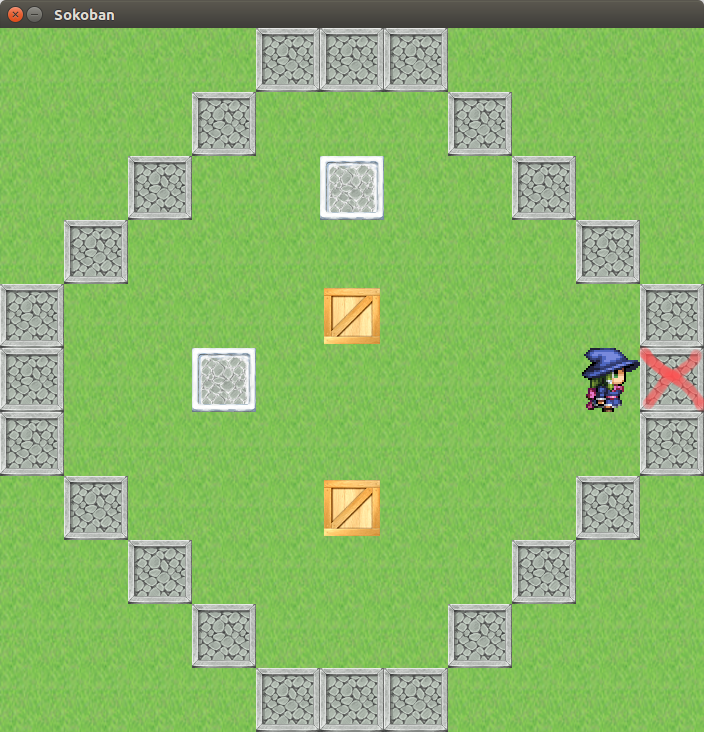
\includegraphics[scale=0.25]{img/01.png}
\caption{Le joueur rencontre un mur, il ne peut pas se déplacer}			
\end{figure}
		\subsubsection{Déplacement des caisses}
Le déplacement des caisses est régie selon les règles suivantes : 
\begin{itemize}
\item Le joueur ne peux pas tirer les caisses, il perd donc d'office la partie s'il pousse une caisse sur une case de coin qui n'est pas une stèle.
\item Le joueur ne peux pousser qu'une seule caisse à la fois.
\end{itemize}		
Dans le même ordre idée que pour la classe \textbf{Personnage}, la classe \textbf{Caisse} est dotée d'une méthode spéciale \textit{déplace()} vérifiant si le déplacement d'une caisse est autorisé, à partir de la position du joueur et de la direction du déplacement demandé. La fonction vérifie d'abord si la prochaine case est bien une caisse et ensuite si la case suivante est une case vide ou une case stèle. Si cette condition est vérifiée le déplacement de la caisse s'effectue comme exposé ci dessous:
\begin{figure}
\begin{center}
\begin{minipage}[b]{0.4\textwidth}
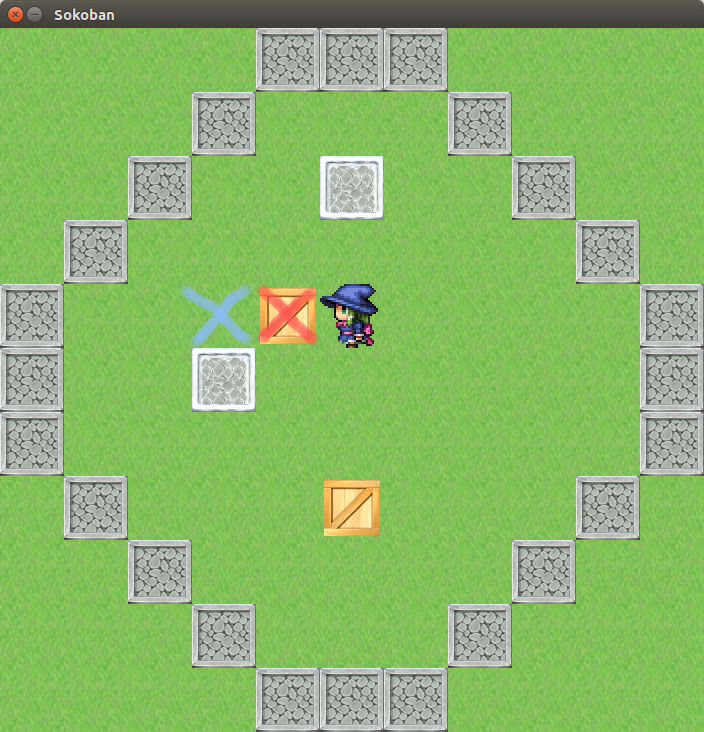
\includegraphics[width=\textwidth]{img/02.png}
\caption{Exemple de déplacement autorisé}
\end{minipage}
\hfill
\begin{minipage}[b]{0.4\textwidth}
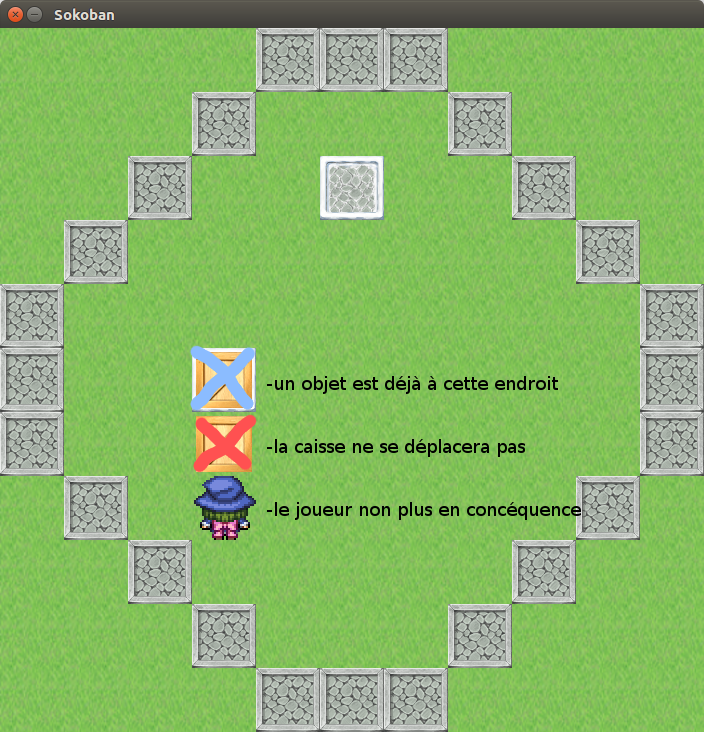
\includegraphics[width=\textwidth]{img/04.png}
\caption{Exemple de déplacement impossible}
\end{minipage}
\end{center}
\end{figure}











\newpage

\section{\underline{ Algorithme de résolution A* et heuristique}}
	
\vspace{1.5 cm}


\subsection{Présentation et objectif:}
L'algorithme A* est un algorithme souvent utilisé pour trouver des chemins dans la résolution de jeux. Il est dans notre cas implémenté sur une grille de Sokoban. En dehors du sokoban où cela nous importe peu, il peut être interrompu pendant son utilisation est relancé plus tard. C'est un algorithme de type "anytime".
Le but de A* est de trouver le chemin \textit{le plus court} pour aller d'un point de départ à un point d'arrivé. Pour cela l'algorithme garde une liste de toutes les étapes futures que l'on appelle "liste ouverte". Cette liste est établie par la fonction g(n). Ensuite, l'algorithme choisit parmi cette liste une étape future qui soit "à priori" la meilleure pour nous mener à l'objectif en un temps qui soit le plus court possible. Pour que cela puisse se faire, nous avons besoin d'une heuristique qui puisse nous aider à déterminer qu'elle est "à priori" la meilleure option. Une fois que cette option est choisie, l'algorithme passe à la "liste fermée". 
\subsection{Explication détaillée avec exemples.}
\subsubsection{Fonctions g et h:}
A chaque étape de l'algorithme, les fonctions g(n) et h(n) sont exécutées pour n étant un point d'arrivé. Cela nous donne les informations suivantes.
\begin{itemize}
\item[• g(n) = Le nombre d'étapes pour aller du point de départ à l'arrivée n.]
\item[• h(n) = L'heuristique qui estime le coup pour aller de n à l'objectif final.]
\item[• f(n) = g(n) + h(n): Le nombre minimum d'étapes si on choisit le point n.]
\end{itemize}
\subsubsection{Etapes détaillées de l'algorithme:}
Voici les étapes de l'algorithme en langage algorithmique: \newline
Soient: OPEN la liste ouvert \newline

Ajouter DEPART à OPEN \newline
Tant que OPEN n'est pas vide:\newline
	Choisir le N ayant le plus petit f(n)\newline
	Si N est l'objectif alors PASS\newline
	Déplacer N dans CLOSED\newline
	Pour chaque N' = PeuBouger(N, direction):\newline
		g(N')=g(N)+1\newline
		h(N')\newline
		Si N' dans OPEN et nouveau N' n'est pas mieux, CONTINUE\newline
		Si N' dans CLOSED and nouveau N' n'est pas mieux, CONTINUE\newline
		supprimer tout N' étant dans OPEN et CLOSED (en même temps)\newline
		Ajouter N comme parent de N'\newline
		Ajouter N' à OPEN\newline
	FIN POUR\newline
FIN TANT QUE\newline
\textit{Si on arrive ici, alors il n'y a pas de solutions.}
			
\subsection{Le cas du Sokoban:}
\subsubsection{Cas général:}
Dans le cas du sokoban, l'heuristique sera le minimum  de déplacements pour atteindre l'objectif si un chemin direct est possible. Or puisque l'on se déplace uniquement à la verticale ou à l'horizontale, cette donnée sera la somme des déplacements horizontaux et verticaux à réaliser.
\begin{center}
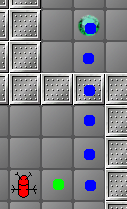
\includegraphics[scale=1]{img/heuristic.png} \newline
\textit{Ce schéma présente le minimum de déplacements pour aller du point rouge au point d'arrivé.}
\end{center}
Ainsi pour l'étape en vert:
\begin{itemize}
\item[g(n)= 1]
\item[h(n)= 6]
\item[f(n)= 1+6 = 7]
\end{itemize}
\subsubsection{Implémentation:}
Tout d'abord, nous avons besoin d'une structure pour les noeuds: \newpage
class Node implements Comparable {\newline
public Node parent;\newline
public int move;\newline
public Location where;\newline
public int g;\newline
public int h;\newline
public int f(){return g+h;}\newline
public Node(Location where, Node parent, int move);\newline
public int compareTo(Object o);\newline
}\newline

Tout d'abord, il est plus pratique de garder la liste OPEN triée pour que l'on puisse avoir facilement accès à notre meilleur option. Il faut donc s'assurer que lorsqu'on ajoute un terme à la liste, celle-ci soit triée automatiquement  \newline
Ensuite il est efficace que nous puissions trouver des noeuds de la liste grâce à l'heure position sur la grille. Cela pour que nous puissions déterminer si 'n' est déjà dans OPEN ou dans CLOSE.


	\newpage	
		
		
		
\begin{center}
	\section{\underline{Schéma UML : diagramme de classe}}
\end{center}
\begin{center}
\vspace{ 4 cm}
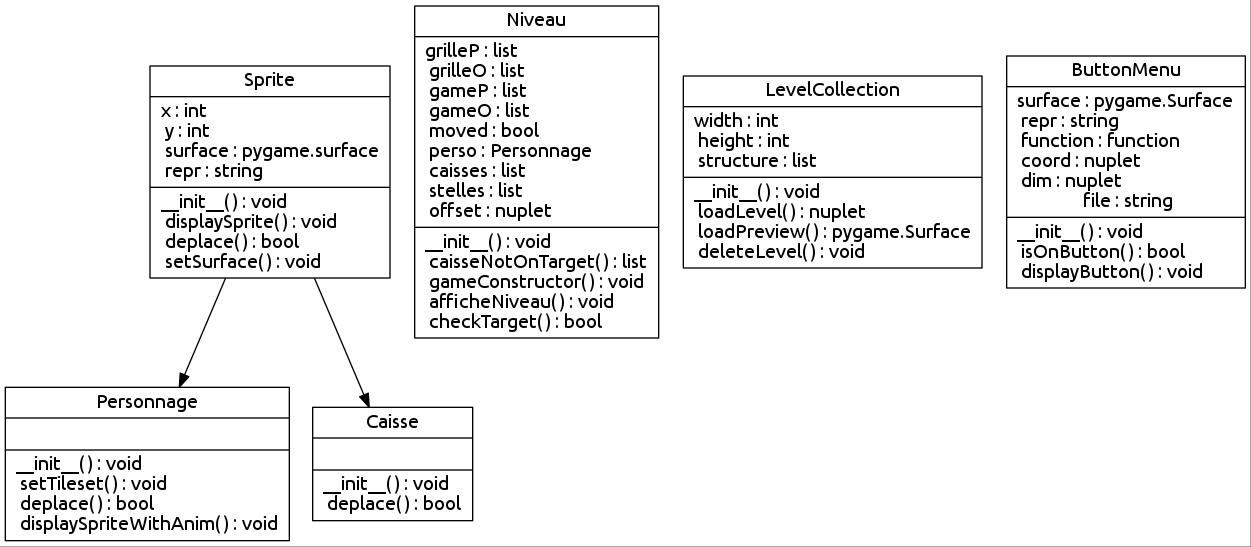
\includegraphics[scale=0.4]{img/dia.jpg}
\end{center}
\newpage

\begin{center}
\section{\underline{Tests de fonctionnalité}}
\end{center}
	\vspace{2cm}
	Une batterie de tests on été effectués via la fonction assert() pour vérifier la fonctionnalité du programme:
\vspace{1cm}
	\begin{itemize}

	\item tests sur classe LevelCollection
		\begin{itemize}
		\item Aux extrêmes: grille de 99999999x99999999 -> erreur out of range
		\item grille unitaire :grille 1x1 -> fonctionnel
		\end{itemize}
		\vspace{0.5cm}
	\item tests sur classe Niveau
		\begin{itemize}
		\item test sur grille incompatible (blocs différents aux même coordonnées) --> erreur lors des test de déplacement liés aux joueurs
		\item test sur des grilles Plan et Obstacle de différentes taille -> erreur out of range si le personnage sort de la première grille
		\end{itemize}
		\vspace{0.5cm}
	\item tests sur le module Astar
		\begin{itemize}
		\item lancement avec un nombre de caisse supérieur a celui des stelles  -> arrêt lorsque plus de stelle disponible
		\item test avec caisse inaccessible sur le niveau "niveautest1.slc" -> erreur
		\item test sur niveau sans caisse -> retourne false(pas une erreur)
		\item test sur niveau sans stelle -> retourne false (pas une erreur) 
		\end{itemize}
	\end{itemize}
\newpage
	
	\begin{center}

	\section{\underline{Tests de performance de la résolution automatique}}
	\vspace{1 cm}
	L'heuristique utilisée effectuant tout les cas possibles , l'exécution de la résolution automatique s'avère très longue dans la plupart des niveaux proposées. Nous avons effectués des tests afin d'obtenir une ordre d'idée des capacités de l'algorithme sur plusieurs niveaux :
	\end{center}
	\vspace{2 cm}
	
\begin{tabular}{|l || c | c |}
\hline
  Nom du niveau & score de difficulté & temps de résolution de l'algorithme \\
 \hline
 \hline
 & &\\
 Aruba Eri & 125 & 9 secondes  \\
  & &\\
  \hline
  & &\\
 AC Easy& 148 & 30 minutes(environ) \\
  & &\\
  \hline
  & &\\
 AC DIAMOND& 1170 & INDETERMINÉ(>5 heures) \\
  & &\\
  \hline
  & &\\
 Amazing 0& 6722 & INDETERMINÉ (>5 heures)\\
  & &\\
 \hline
 \end{tabular}
\vspace{1cm}



Le score de difficulté est déterminé par ((le nombres de cases vides - le nombre d'obstacle) * le nombres de caisse a placer pour compléter le niveau). Les niveaux dont le temps de résolution est indéterminé on été soumis a l'exécution d'astar pendant plus de 5 heures au minimum , sans résultats .

 
 









\end{document}